% !TEX program = lualatex
\documentclass[a4paper,12pt]{article}

\usepackage[brazil]{babel}
\usepackage{geometry}
\geometry{top=2.5cm,bottom=2.0cm,left=2.5cm,right=2.0cm}

% Matemática / tabelas
\usepackage{amsmath}
\usepackage{amssymb}
\usepackage{amsthm}
\usepackage{array}
\usepackage{booktabs}
\usepackage{multirow}
\usepackage{multicol}
\usepackage{tabularx}
\usepackage{makecell}
\usepackage{siunitx}
\usepackage{lipsum}

% Listas e floats
\usepackage{enumitem}
\usepackage{float}

% Figuras
\usepackage{graphicx}
\usepackage[table]{xcolor}

% Fonte (LuaLaTeX)
\usepackage{fontspec}
\setmainfont{Times New Roman}

% Microtipografia / links / PDFs
\usepackage{microtype}
\usepackage{hyperref}
\usepackage{pdfpages}

% Caption
\usepackage[hypcap=false]{caption}

% TikZ/PGFPlots
\usepackage{pgfplots}
\usepackage{pgfplotstable}
\pgfplotsset{compat=1.18, width=11cm}
\usepgfplotslibrary{fillbetween}
\usetikzlibrary{calc,arrows.meta,intersections,decorations.pathreplacing}

% Bibliografia ABNT
\usepackage{csquotes}
\usepackage[
  backend=biber,
  style=abnt,
  sorting=nyt
]{biblatex}
\addbibresource{referencias.bib}

% Ambientes
\theoremstyle{definition}
\newtheorem{example}{Exemplo}[section]

\theoremstyle{definition}
\newtheorem{propriedade}{Propriedade}[section]

\theoremstyle{definition}
\newtheorem{definicao}{Definição}[section]

% Listas
\setlist[itemize]{noitemsep,topsep=4pt}

\begin{document}

\tableofcontents
\newpage

\section{Introdução}

\begin{table}[hbt]
    \centering
    \begin{tabular}{lll}
        \toprule
        \multicolumn{3}{c}{\textbf{ROCHAS SEDIMENTARES}} \\
        \midrule
        Clásticas            &                            & Não clásticas \\
        Vulcanoclásticas     &                            & Carbonatos \\
                             & $\hookrightarrow$ Turfas   & Evaporitos \\
                             & $\hookrightarrow$ Argilitos & Outros \\
        Terrígenas           &                            & \\
        Carbonáticas (CaCO$_3$) &                        & \\
        \bottomrule
    \end{tabular}
    \caption{Rochas sedimentares}
    \label{tab:sedimentares}
\end{table}

\subsection{Esquemático de uma bacia de sedimentação}

\begin{figure}[hbt]
    \centering
    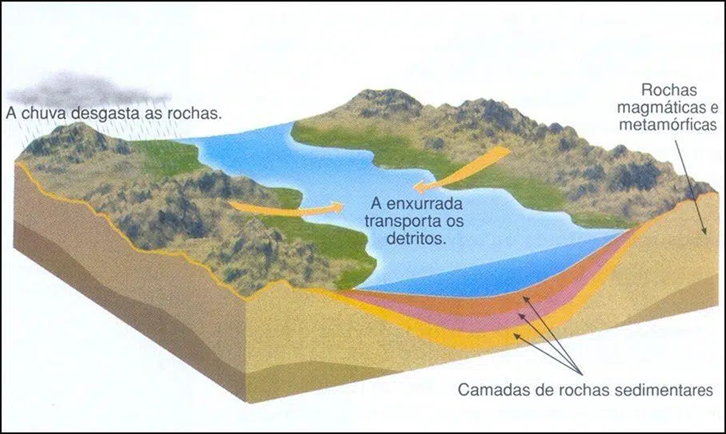
\includegraphics[width=0.8\linewidth]{Figs/bacia_sedimentar.png}
    \caption{Esquema de uma bacia de sedimentação}
    \label{fig:bacia_sedimentar}
    
    \caption*{\footnotesize Fonte: elaborado pelo autor com base em \textcite{milhomem2023baciassedimentares}.}
\end{figure}


\begin{definicao}
Bacia sedimentar é uma depressão tectônica ou região da crosta em subsidência na qual ocorre acumulação prolongada de sedimentos, posteriormente preservados no registro geológico e, na maioria, transformados em rochas sedimentares por compactação e litificação. Diferentemente da simples bacia de sedimentação, que enfatiza o espaço de deposição, a bacia sedimentar corresponde à unidade geológica já caracterizada pelo preenchimento sedimentar.
\end{definicao}

Então a formação de rochas clásticas se inicia na fragmentação que ocorre nas regiões de soerguimento pela ação dos inteperísmos, transportados pelos agentes de transporte e aculumulação na bacia de sedimentação.

São formados:

\begin{enumerate}[label=\alph*.]
    \item Evaporitos,
    \item Carbonatos,
        \begin{itemize}
            \item Sulfatos,
            \item Cloritos.
        \end{itemize}
\end{enumerate}

Outras rochas sedimentares
\begin{enumerate}[label=\alph*.]
    \item Carvão,
    \item Ironstones
    \item Depósitos silicosos
\end{enumerate}

\section{Rochas sedimentares}
\subsection{Rochas Sedimentares}

\begin{definicao}
    
Granulometria é a distribuição dos tamanhos dos grãos ou partículas que compõem um material. Uma de suas formas de determinação é o peneiramento, no qual a amostra é submetida a uma série de peneiras com aberturas de malha conhecidas, ficando retidas em cada peneira as partículas com dimensões superiores à respectiva abertura e inferiores à da peneira imediatamente anterior.
    \end{definicao}
Em relação à granunlometria podemos primariamente classificar os como:
\begin{enumerate}
    \item Grossos,
    -- 2,0 mm
    \item Areia, e
    -- 0,0625 mm
    \item Finos (Silte/argila)
    -- 0,0039 mm
\end{enumerate}

\begin{definicao}
Rochas clásticas são rochas sedimentares detríticas constituídas por fragmentos de minerais, rochas ou restos preexistentes, gerados por intemperismo, erosão, transporte, deposição e posterior litificação. Sua classificação baseia-se, em geral, no tamanho, na composição e no grau de seleção dos clastos.
\end{definicao}

\begin{definicao}
Rochas terrígenas são rochas sedimentares formadas a partir de sedimentos provenientes do retrabalhamento de áreas continentais emersas ou próximas ao continente. O termo enfatiza a proveniência do material detrítico, isto é, sua origem terrestre ou continental.
\end{definicao}

\begin{definicao}
Rochas siliciclásticas são rochas sedimentares detríticas compostas predominantemente por clastos de minerais silicáticos e fragmentos líticos, como quartzo, feldspatos e fragmentos de outras rochas. O termo enfatiza a natureza composicional dos sedimentos, marcada pelo predomínio de silicatos.
\end{definicao}

As rochas siliciclásticas constituem, em geral, a principal categoria das rochas terrígenas, pois grande parte dos detritos oriundos do continente é composta por minerais silicáticos. Assim, embora os termos terrígena e siliciclástica frequentemente coincidam no uso corrente, não são rigorosamente sinônimos: o primeiro destaca a origem do material, enquanto o segundo destaca sua composição.

Podemos classificas rochas sedimentares como:
\begin{enumerate}
    \item Conglomerados,
    \item Arenitos, e
    \item Pelitos que,
    podem ser subdivididos em;
        \begin{enumerate}
            \item Argilitos,
            \item Siltitos,
            \item Lamitos, e
            \item Folhelhos
        \end{enumerate}
\end{enumerate}

\printbibliography

\end{document}